\documentclass{article}

% Listings
\usepackage{listings}
\usepackage{color}
\usepackage{upquote} % preserve backticks

% Syntax highlighting
\usepackage{minted}
\usemintedstyle{tango}

% Fonts
%\usepackage{palatino}
\usepackage{inconsolata}
\usepackage[T1]{fontenc}

% Margin
\usepackage[margin=0.5in]{geometry}

% Images
\usepackage{graphicx}
\graphicspath{ {images/} }


% Colors
\definecolor{comment}{rgb}{0.31,0.31,0.31}
\definecolor{codegray}{rgb}{0.19,0.19,0.19}
\definecolor{string}{rgb}{0.56,0.66,0.35}
\definecolor{backcolor}{rgb}{0.96,0.96,0.96}
\definecolor{keyword}{rgb}{0.67,0.25,0.25}
 
\lstdefinestyle{mystyle}{
    backgroundcolor=\color{backcolor},
    commentstyle=\color{comment},
    keywordstyle=\color{keyword},
    numberstyle=\tiny\color{codegray},
    stringstyle=\color{string},
    basicstyle=\footnotesize\ttfamily,
    breakatwhitespace=false,
    breaklines=true,
    captionpos=t,
    keepspaces=true,
    numbers=left,
    numbersep=5pt,
    showspaces=false,
    showstringspaces=false,
    showtabs=false,
    tabsize=2
}

\lstset{style=mystyle}

\definecolor{bg}{rgb}{0.95,0.95,0.95}
\newmintedfile{c}{linenos,bgcolor=bg,fontfamily=sourcecodepro}
\newmintedfile{bash}{linenos,bgcolor=bg,fontfamily=sourcecodepro}




\title{Homework 1 - Virtual Machine Scheduling Analysis}
\author{Jared Klingenberger}
\date{February 8, 2016}

\begin{document}

\maketitle

\lstlistoflistings

\section{Rosenblum Paper}

To summarize, Rosenblum's paper on virtual machines is a good overview of the
numerous motivations behind virtual machines. In the early days of virtual
machine computing, a big motivation was for compatibility between different
types of hardware by having a single target abstract machine to code to.
However, a different style of virtual machine made a huge comeback in recent
years with the arrival of VMWare, a hardware-level virtual machine that made it
possible to emulate computer hardware devices. This is quite useful for many
reasons; two such reasons are that these VMs provide superior isolation and that
one can manage the execution of these VMs from a higher level with a Virtual
Machine Manager.

\section{Manual Dataset Creation and Analysis}

Overall for question 2, I noticed that as I increased the blocksize, there
seemed to be noticeable periodic effects in the datasets. So most of the results
would fall around the same value, but some delays were much longer and stacked
around the same times. This likely has something to do with how the scheduler
assigns clock time to different processes. The most noticeable effect can be
seen with blocksize of 1 million.

\subsection{Statistics}

Here are histogram plots and numerical statistics for different blocksizes.

\subsubsection{Blocksize 4}

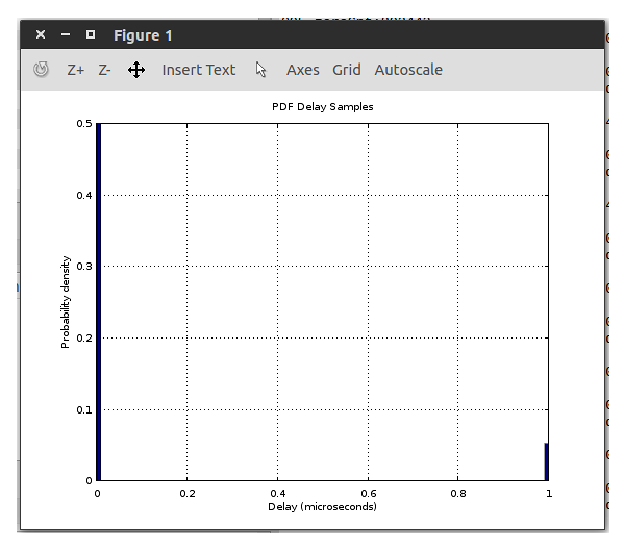
\includegraphics{q2/hw1-4}

\begin{lstlisting}
plotDataPDF (nargin:1):  sampleSize:1000000, maxValue:65.100000,  MAX_ALLOWED_VALUE:1000.000000
#samples:1000000 Mean:     0 microseconds,  median:      0,  std:      0, max:    65, min:     0, maxCount:10173 zeroCnt:947490
percentiles (2.5 25 50 75 97.5): :     0      0      0      0      1
\end{lstlisting}

\subsubsection{Blocksize 256}

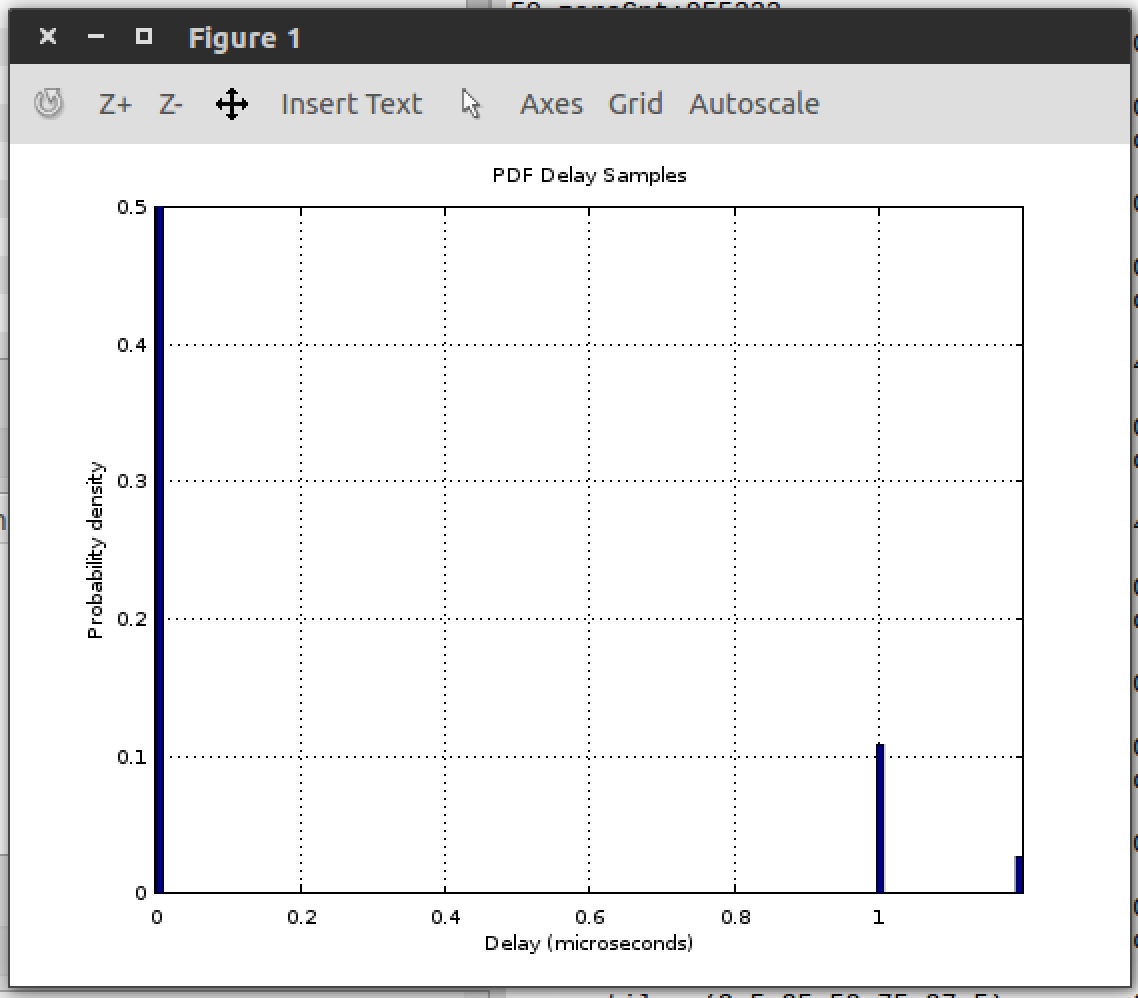
\includegraphics{q2/hw1-256}

\begin{lstlisting}
plotDataPDF (nargin:1):  sampleSize:1000000, maxValue:70.100000,  MAX_ALLOWED_VALUE:1000.000000
#samples:1000000 Mean:     0 microseconds,  median:      0,  std:      0, max:    70, min:     0, maxCount:235 zeroCnt:865266
percentiles (2.5 25 50 75 97.5): :     0      0      0      0      1
\end{lstlisting}

\subsubsection{Blocksize 65535}

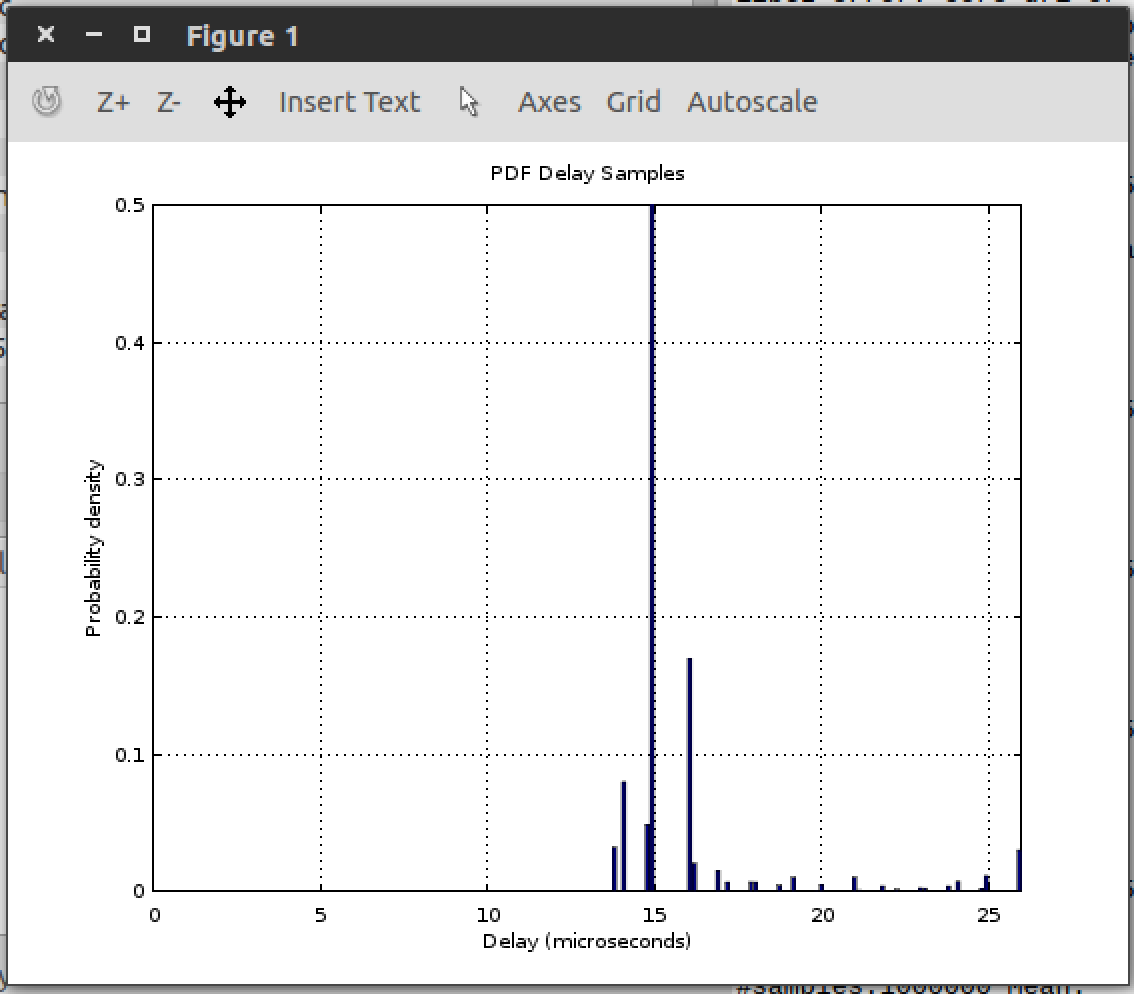
\includegraphics{q2/hw1-65535}

\begin{lstlisting}
plotDataPDF (nargin:1):  sampleSize:1000000, maxValue:4635.100000,  MAX_ALLOWED_VALUE:1000.000000
#samples:1000000 Mean:    16 microseconds,  median:     15,  std:      7, max:  4635, min:    12, maxCount:22358 zeroCnt:0
percentiles (2.5 25 50 75 97.5): :    14     15     15     16     26
\end{lstlisting}

\subsubsection{Blocksize 1000000}

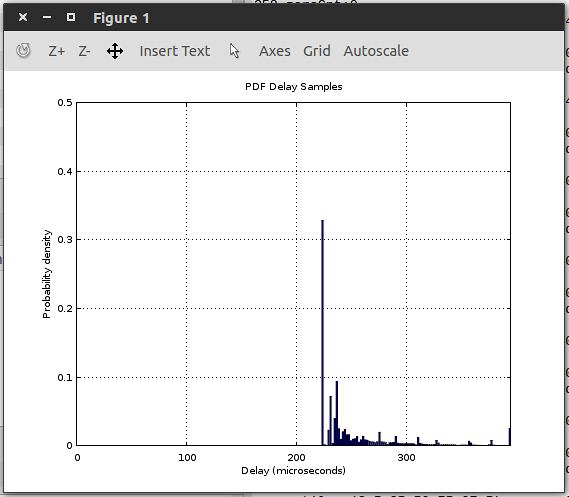
\includegraphics{q2/hw1-1000000}

\begin{lstlisting}
plotDataPDF (nargin:1):  sampleSize:1000000, maxValue:5667.200000,  MAX_ALLOWED_VALUE:1000.000000
#samples:1000000 Mean:   255 microseconds,  median:    236,  std:     51, max:  5667, min:   210, maxCount:24825 zeroCnt:0
percentiles (2.5 25 50 75 97.5): :   223    224    236    263    395
\end{lstlisting}

\subsection{Parallel execution}

I think the programs were completing too quickly to affect mpstat, but I was able to see a spike in CPU usage through using the `top` command.

\begin{lstlisting}
11:30:35 PM  CPU    %usr   %nice    %sys %iowait    %irq   %soft  %steal  %guest  %gnice   %idle
11:30:35 PM  all    0.38    0.00    0.03    0.00    0.00    0.00    0.00    0.00    0.00   99.58
11:30:35 PM    0    0.46    0.00    0.05    0.00    0.00    0.00    0.00    0.00    0.00   99.48
11:30:35 PM    1    0.34    0.01    0.03    0.00    0.00    0.00    0.00    0.00    0.00   99.62
11:30:35 PM    2    0.35    0.00    0.03    0.00    0.00    0.00    0.00    0.00    0.00   99.62
11:30:35 PM    3    0.36    0.00    0.02    0.01    0.00    0.00    0.00    0.00    0.00   99.61
\end{lstlisting}

\section{Experiments in Parallel VM Scheduling}

Blah blah blah

\subsection{Experiment 1}

This is exp1

\subsection{Experiment 2}

This is exp2

\subsection{Experiment 3}

This is exp3

\section{Code}

\lstinputlisting[language=c,caption=hw1.c,frame=single,label=code:hw1]{hw1.c}

\lstinputlisting[language=bash,caption=runHW1.sh,frame=single,label=code:runHW1]{runHW1.sh}

\lstinputlisting[language=bash,caption=analysisHW1.sh,frame=single,label=code:analysisHW1]{analysisHW1.sh}

\lstinputlisting[language=awk,caption=analyzeResults.awk,frame=single,label=code:analyzeResults]{analyzeResults.awk}

\end{document}